\section{Empirical results}
\label{sec:empirical-results}
To evaluate the algorithms presented in Section~\ref{sec:flexible-resource-allocation-mechanisms}, we analyse the performance of  the greedy and the  auction algorithms (Subsections~\ref{subsec:evaluation-of-the-greedy-algorithm} and~\ref{subsec:evaluation-of-the-auction-mechanisms}). We also investigate a range of server heuristics on the decentralised iterative auction (Subsection~\ref{subsec:decentralised-iterative-auction-heuristics}) and the ability to profit by misreporting task attributes within the decentralised iterative auction (Subsection~\ref{subsec:dia-misreport-task-attributes}). Finally, we analyse the effect of server resource capacity ratios on performance (Subsection~\ref{subsec:server-resource-capacity-ratio}).

Within Edge Cloud Computing, we have found no \emph{de facto} standard for testing resource allocation algorithms and those used in related work have unique models that do not consider a deadline that is applicable to our work. Therefore, we have generated synthetic models for both our servers and tasks with a Gaussian distribution for each attribute. This model can be found in Section 6 of the supplementary material. 

The model settings chosen to test are 2 servers and 10 tasks, 3 servers and 15 tasks, 6 servers and 30 tasks and 8 servers and 40 tasks. In all of these cases, around 70\% of tasks are allocated. To compare to previous work, that utilise a fixed resource requirement, each task's resource speeds were determined prior to running the algorithms by finding the minimum total sum of resource speeds according to the task deadline. This aims to give each task a balanced amount of each resource to make comparisons as fair as possible.

To find the optimal solution of the optimisation problem, from Subsection~\ref{subsec:optimisation-problem}, a mixed integer linear programming algorithm is used. However, due to the difficulty of finding the optimal solution, \textcolor{black}{this was only used in smaller settings where the optimal can be found within a reasonable amount of time}. 

\begin{figure*}[t]
    \centering
    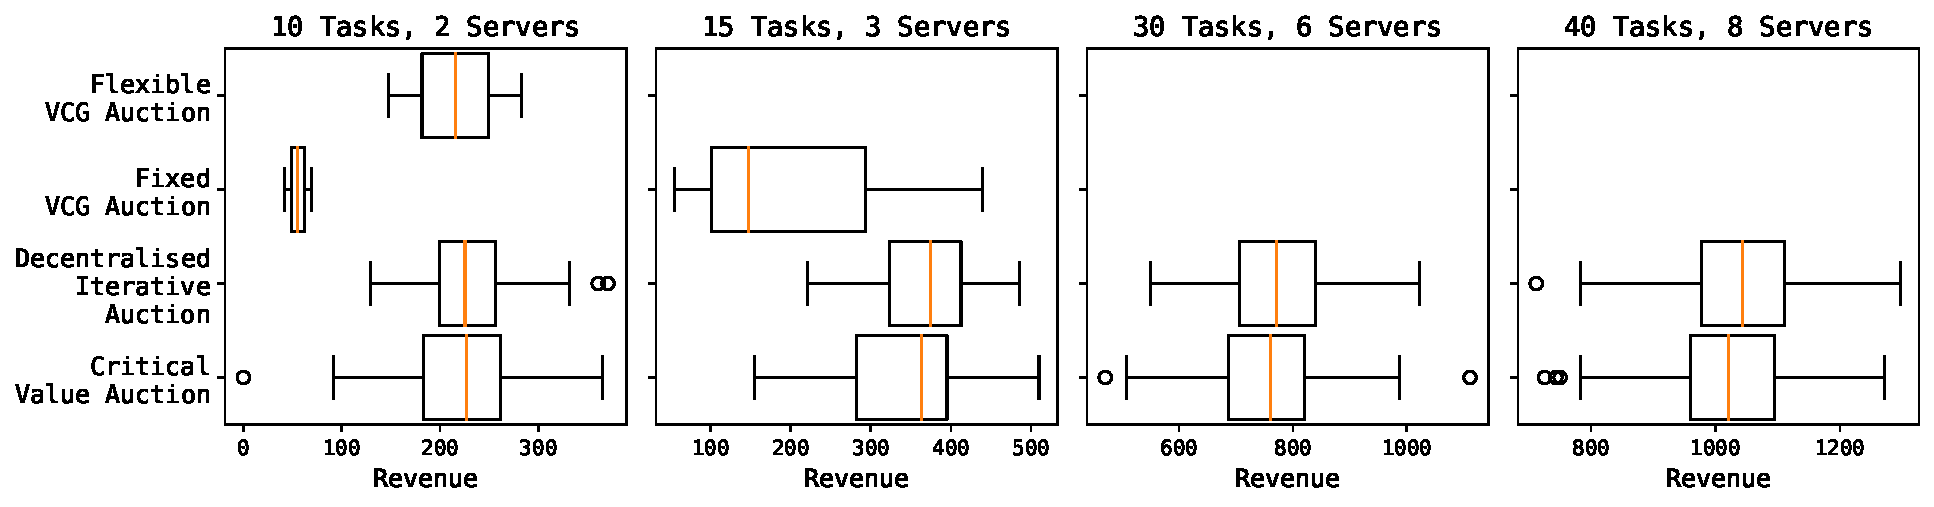
\includegraphics[width=\textwidth]{figs/auctions/revenue.pdf}
    \caption{Revenue of the flexible VCG auction, fixed VCG auction, decentralised iterative auction and critical value auction for a range of model settings.}
    \label{fig:auction-mechanisms-revenue}
\end{figure*}

\begin{figure*}[b]
    \centering
    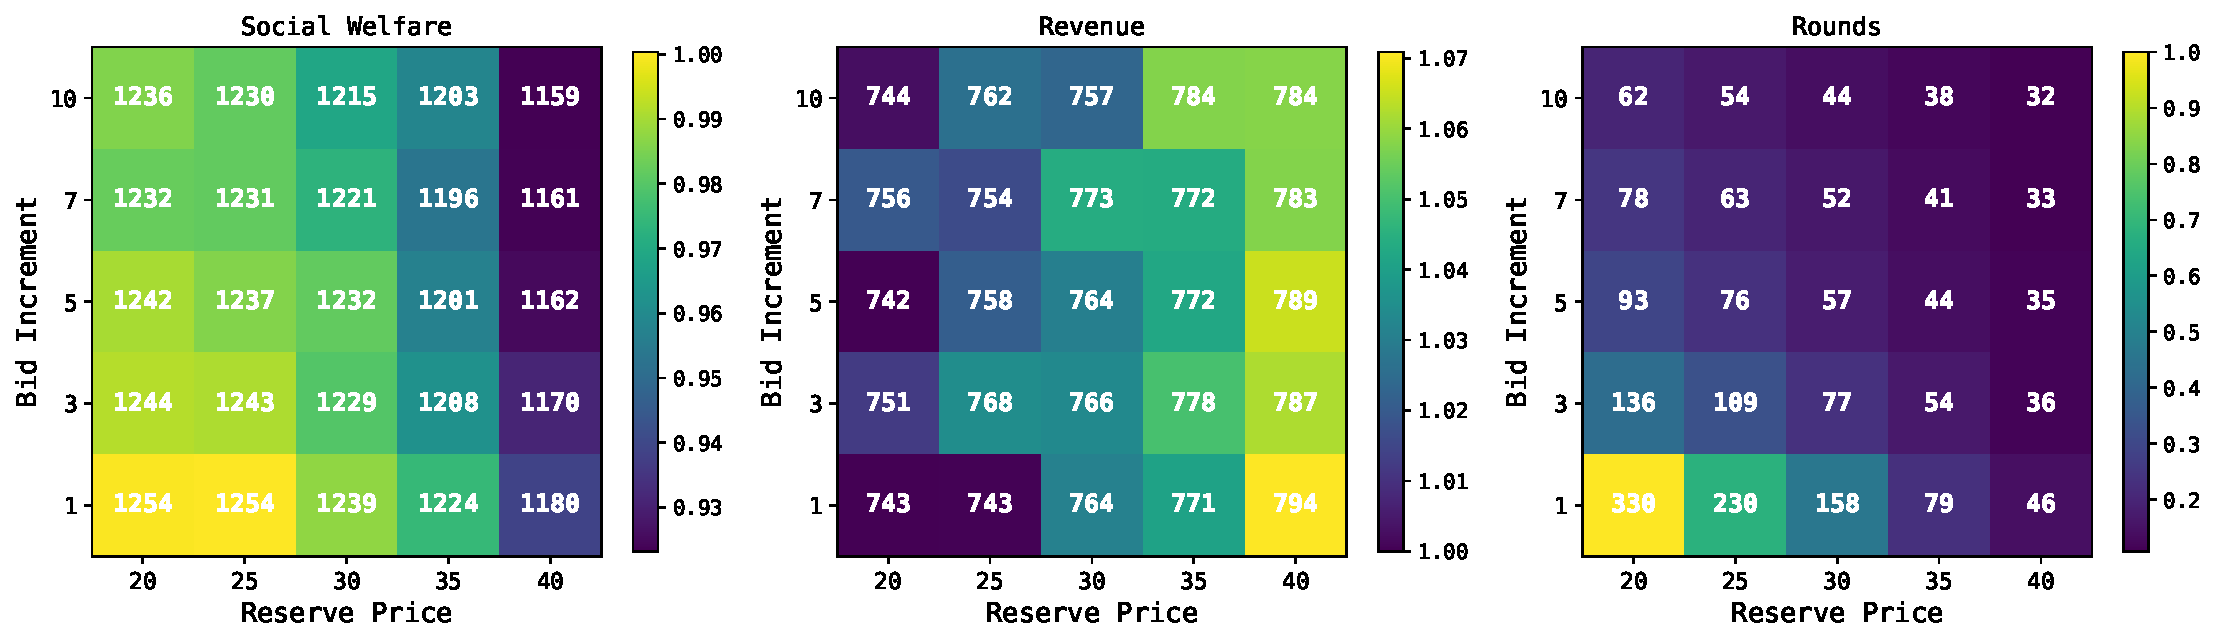
\includegraphics[width=\textwidth]{figs/dia_heuristics/grid_search.pdf}
    \caption{Average social welfare, revenue and rounds for different bid increments and initial cost heuristics of the decentralised iterative auction.}
    \label{fig:dia-heuristic-search}
\end{figure*}

\subsection{Evaluation of the greedy algorithm}
\label{subsec:evaluation-of-the-greedy-algorithm}
Due to the complexity of the optimisation problem, for the larger settings, it is not possible to get the optimal solution. Therefore, we implemented a relaxed version of the problem for comparisons with the optimal solution in larger cases. The relaxed version differs from our standard optimisation problem as there exists a single ``super'' server where its resources are the sum of the original servers' resource capacities. The formal relaxed optimisation problem can be found in Section 5 of the supplementary material. 

For the greedy algorithm, a wide range of possible heuristics were tested with the best found being - task priority: $\frac{v_j \cdot d_j}{s_j + w_j + r_j}$, server selection: $\text{argmin}_{\forall i \in I} S^{'}_i \cdot W^{'}_i \cdot R^{'}_i$ for task $j$ and servers $I$ and the resource allocation: \[\text{argmin}_{s^{'}_j, w^{'}_j, r^{'}_j} \left(\frac{w^{'}_j}{W^{'}_i}\right)^3 + \left(\frac{s^{'}_j + r^{'}_j}{R^{'}_i}\right)^3\] for task $j$ and server $i$. Using this task priority function means that the lower bound in Subsection~\ref{subsubsec:greedy-lower-bound} does not  hold.  However, these functions achieve better results due to considering more task attributes. In our future work, we are planning to explore the ability to use machine learning to find better functions.

Figure~\ref{fig:greedy-algorithm-comparison} shows the social welfare achieved by the four algorithms over  four different settings. As can be seen from Figure~\ref{fig:greedy-algorithm-comparison}, the greedy algorithm and the optimal flexible solution provide similar results, with the percentage difference being  between 98.4\% and 97.6\% for the first two cases, respectively. The overall percentage difference between the optimal flexible and fixed resource allocation mechanisms is 83.4\% and 73.7\%, while the percentage difference between the greedy algorithm and the optimal relaxed solution is 93.7\%, 95.0\%, 91.8\%, and 92.3\%. These results show the consistency of the algorithms even in larger settings and that our flexible resource allocation achieves around 20\% better performance than prior work. 

\subsection{Evaluation of the auction mechanisms}
\label{subsec:evaluation-of-the-auction-mechanisms}
The Vickrey-Clarke-Groves (VCG) mechanism \cite{vickrey,Clarke,groves} is a standard method of dealing with self-interested users, as it is strategyproof. However, this requires solving the optimal solution for each individual task, making such a mechanism infeasible except for small settings. Therefore, VCG is used for a comparison with the critical value auction and decentralised iterative auction in the smaller settings.

For the critical value auction, the same functions are used for the analysis of the greedy algorithm (Subsection~\ref{subsec:evaluation-of-the-greedy-algorithm}). For the decentralised iterative auction, the server heuristics used are a bid increment of 3 and a reserve price of 25 for all servers. The reason for these heuristics over others is explained in Subsection~\ref{subsec:decentralised-iterative-auction-heuristics}.

Figure~\ref{fig:auction-mechanisms-revenue} plots the revenue achieved by the auction mechanisms across different settings. This shows that both the critical value auction and the decentralised iterative auction achieve comparable results, being within 4\% of each other for all of the settings. The figure for the social welfare achieved by the auction mechanisms can be found in Section 7 of the supplementary material. For the critical value auction, it achieves 101.3\%, 97.2\%, 97.1\%, 97.3\% percent difference in social welfare compared to the decentralised iterative auction.

\subsection{Decentralised iterative auction heuristics}
\label{subsec:decentralised-iterative-auction-heuristics}
As explained in Subsection~\ref{subsec:decentralised-iterative-auction}, the decentralised iterative auction uses two heuristics for calculating the price of a task; bid increment and a reserve price. We investigated a selection of different bid increment and reserve price heuristics to compare social welfare, revenue and total rounds required. The reserve prices used are 20, 25, 30, 35 and 40, while the bid increments are 1, 3, 5, 7 and 10. The mean value of tasks is 50 (see Section 6 of the supplementary material for task model attributes). For the experiment, 30 tasks and 6 servers were used.

% An example to show this is if a task has a value of 10 and the difference in server revenue is 7. In this case, if the server's bid increment is 4, the resulting price is 11, above the task's value prevent it from being allocated. However if the server's bid increment was 3 then the task could have been allocated. A similar such problem exists for the server's reserve price as the server if the reserve price is above task's value then the task could never be allocated to the server. Therefore it is extremely important for both the server and tasks that the servers' heuristics are efficient allowing for tasks to be allocated to  servers. 

Figure~\ref{fig:dia-heuristic-search} shows the social welfare, revenue and required rounds for the grid search over server heuristics with values normalised by the bid increment of 1 and reserve price of 20. For the social welfare, it is consistent with just a 7\% difference in social welfare from the worst heuristics (bid increment of 10 and reserve price of 10) and the best heuristics (bid increment of 1 and reserve price of 20). This resilience is important as even if the servers choose high bid increments or reserve prices, the social welfare of the system is not significantly affected. 

For the revenue, the lowest revenue occurs for the case of price change of 1 and reserve price of 20, which has the best social welfare. The reason for this occurring is due to how the auction ends, either when all tasks are allocated to a server or can't be allocated to a server. This is because the reserve price causes the winning price of tasks to be inflated, meaning that the highest revenue has a bid increment of 1 and a reserve price of 40.  
 
Within the context of edge cloud computing, the time it takes for the auction to run is an important attribute. For the auction, we define a round as task advertising to all of the servers. The third graph shows the average number of rounds required for each heuristic to converge to a price. For the smallest heuristics (a bid increment of 1 and reserve price of 20), this achieves the highest social welfare. However, this comes at the cost of requiring on average 330 rounds. This means that on average each task requires 11 individual rounds to converge to a price. In comparison, when the bid increment is 10 and the reserve price is kept at 20, the average number of rounds required is 80 ($5\times$ less), with each task requiring on average two advertisements.

Figure~\ref{fig:dia-heuristic-search} collectively shows that it is an effective auction but it has trade-offs with each heuristic being selected with regards to social welfare, revenue and time taken. 

\subsection{Misreporting task attributes in the decentralised iterative auction}
\label{subsec:dia-misreport-task-attributes}
In Subsection~\ref{subsec:decentralised-iterative-auction}, the decentralised iterative auction was shown to not be incentive compatible in particular cases. However, it was unknown how often tasks could profit from misreporting and by how much. To test this, we used 6 servers and 30 tasks with server heuristics having a bid increment of 3 and  reserve price of 25.

Due to the inherent randomness of the auction, as the system does not have a central auctioneer, the final prices that tasks receive can vary. We found that when the auction is repeatedly run, the allocation of tasks to servers along with the price was not consistent each time. Therefore, there is a problem with analysing the ability for tasks to misreport task attributes as if a task does better or worse. This cannot be easily determined because of the change in task price.

We ran a grid search of possible attributes within 10\% of the original value for an individual task to check the most plausible misreported versions of a task to find if the task would be allocated or even achieve a lower (better) price than the original truthfully reported version of the task. We found that in testing 10 tasks, most of the misreported tasks could still be allocated; 6 tasks were allocated 100\% of the time and the rest of them were allocated 0\%, 0\%, 60.3\% and 99\%, respectively. Despite this, only 4 tasks were able to achieve a better price with a misreported version, for 2\%, 4.7\%, 37.4\% and 29.7\% of the time. The reason for such a high variability in misreporting ability is due to the original truthful auction giving the task a price larger than it is  plausible. %% TODO This was confirmed but repeating the auction with the same truthful attributes where the task prices achieved being lower than the original price

\subsection{Impact of server resource capacity on resource allocation}
\label{subsec:server-resource-capacity-ratio}
Within edge cloud computing, nodes may have a large discrepancy in server resource capacity compared to task requirements for several reasons: a persistence task running over a long period of time, internet connection issues limiting overall bandwidth, etc. Therefore, we compare the performance of our elastic resource allocation to fixed resource allocation by redistributing server computation and bandwidth capacities with different ratios. \footnote{The server storage is ignored here as there is no flexibility in the storage usage.} For this experiment we use 15 tasks and 3 servers.

\begin{figure}[ht]
    \centering
    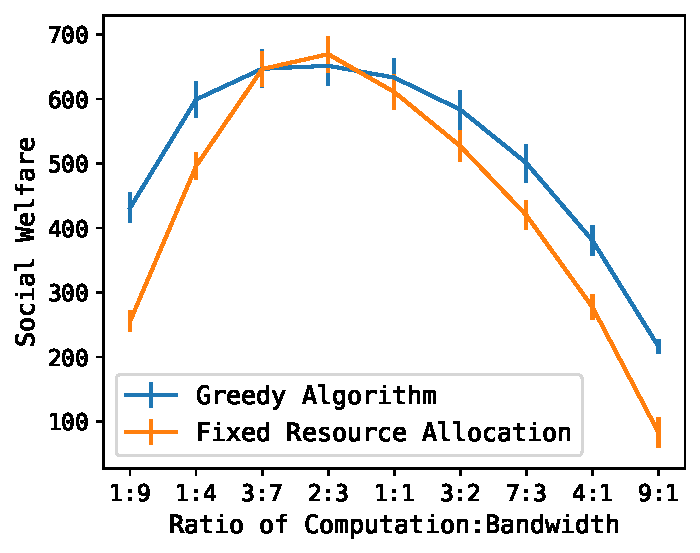
\includegraphics[width=\linewidth]{figs/resource_ratio/social_welfare.pdf}
    \caption{Social welfare of greedy algorithm and optimal fixed solution for redistributed server resource capacity ratios.}
    \label{fig:resource-ratio-social-welfare}
\end{figure}

Figure~\ref{fig:resource-ratio-social-welfare} shows the average social welfare achieved by the respective algorithms with different server resource ratios. As can be seen on the figure at the ratio extremes, there is a significant difference in results between the greedy algorithm and fixed resource allocation. This difference in social welfare is up to 50\% for the most extreme cases while for the cases where the server resource are distributed then the performance difference is with 95\% confidence interval. The reason for the ability of the flexible resource allocation be able to achieve better social welfare in these extreme cases is as control of allocating resources has shifting from tasks to servers. 